\documentclass{szzclass}
\usepackage[czech]{babel}
\usepackage{dependencies/szz-code}
\usepackage{hyperref}

\title{Čisté objektové paradigma — principy návrhu OO systémů.}

\begin{document}
\maketitle

\tableofcontents
\newpage

\section{Postup návrhu OO systémů}

\begin{enumerate}
      \item Identify minimal requirements
      \item Make requirements testable
      \item Identify objects and their responsibilities
      \item Implement and test classes
      \item Refactor to simplify design
      \item Iterate
\end{enumerate}

\section{Povinosti objektů}

\begin{itemize}
      \item uchovávat informace a poskytovat služby pracující s těmito informacemi
      \item \textbf{high cohesion} -- vysoká soudružnost operací a dat uvnitř třídy
      \item \textbf{low coupling} -- nízká provázanost mezi třídami
      (\textit{Každá třída by měla provádět právě jednu činnost})
      \item \textbf{high-level-of-abstraction} -- vysoká míra abstrakce.
      Na všechno mít speciální rozhraní a vždy používat rozhraní místo implementace.
\end{itemize}


\section{Symptomy degradujícího návrhu SW}

\begin{itemize}
      \item \textbf{Rigidity} -- SW není snadné jednoduše měnit nebo rozšiřovat,
      nelze přidávat ani jednoduché funkcionality.
      \item \textbf{Fragility} -- Změna jedné části SW ovlivní (rozbije) jinou
      část SW (třeba i konceptuálně odlišnou).
      \item \textbf{Immobility} -- Není možné znovu použít SW pro jiné projekty
      nebo alespoň pro části jiných projektů.
      \item \textbf{High design viscosity} -- Udržování správného návrhu je implementačně náročnější
      než to udělat proti pravidlům daného návrhu, což vede k degradaci návrhu.
      \item \textbf{High environment viscosity} -- Prostředí pro vývoj SW je pomalé a neefektivní.
      Například dlouhý \textit{compile-time}.
\end{itemize}


\section{Principy OO návrhu}

Dodržování následujících principů vede ke snížení provázanosti mezi třídami.
V přednáškách bylo zmíněných pět principů zaměřených na návrh tříd.
Ostatní principy se týkají rozdělení tříd do balíčků.
Všechny principy OO návrhu lze najít na:

\textbf{http://www.butunclebob.com/ArticleS.UncleBob.PrinciplesOfOod}

\begin{itemize}
      \item \textbf{SRP -- single responsibility principle}
      \textit{A class should have one, and only one, reason to change.}

      Každá třída, modul nebo metoda má mít pouze jednu povinnost, jeden účel.
      Tato povinnost by měla být kompletně zapouzdřena touto třídou, modulem, metodou.

      \item \textbf{OCP -- open-closed principle}

      \textit{You should be able to extend a classes behavior, without modifying it.}

      SW entity by měly být snadno rozšiřitelné, ale nesmí být možnost měnit jejich chování.

      \item \textbf{LSP -- Liskov substitution principle}

      \textit{Derived classes must be substitutable for their base classes.}

      Odvozené třídy musejí být použitelné přes rozhraní jejich nadřazené třídy.
      Uživatel zvenku nezmí poznat rozdíl mezi \textit{derived class} a \textit{base class}.

      \item \textbf{ISP -- interface segregation principle}

      \textit{Make fine grained interfaces that are client specific.}

      Více detailních rozhraní je lepší než jedno obsáhlé rozhraní (\textit{general purpose}).
      Každá třída musí implementovat pouze takové metody, které skutečně používá a potřebuje.
      Nikdy se nesmí stát, že by třída musela kvůli svému rozhraní implementovat něco, co nepotřebuje.
      \begin{figure}[ht]
            \centering
            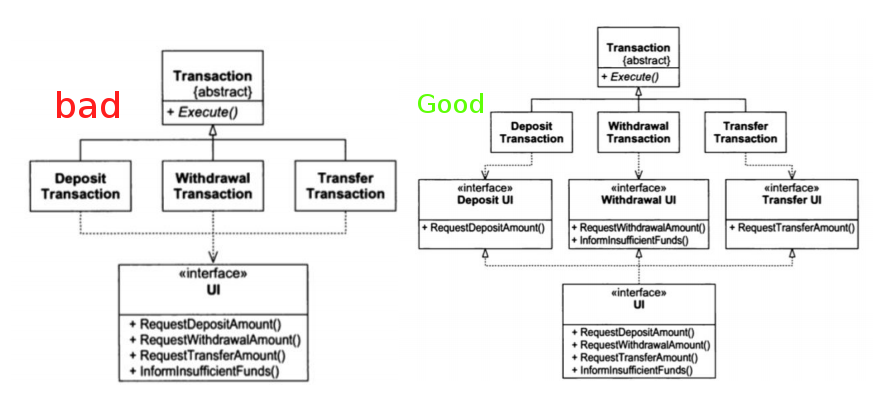
\includegraphics[width=1\textwidth]{topics/bi-wsi-si-09/isp.png}
            \caption{ISP example}
      \end{figure}

      \item \textbf{DIP -- dependency inversion principle}

      \textit{Depend on abstractions, not on concretions.}

      Abstrakce by neměla záviset na detailech. Detaily by měly záviset na abstrakci.
      \begin{figure}[ht]
            \centering
            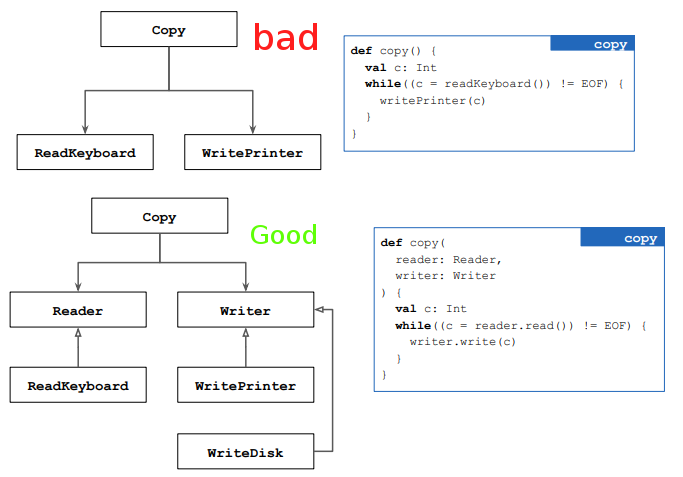
\includegraphics[width=1\textwidth]{topics/bi-wsi-si-09/dip.png}
            \caption{DIP example}
      \end{figure}


\end{itemize}

\section{Závěr k principům OO návrhu}

Malé shrnutí z přednášky o principech OO návrhu:

\begin{itemize}
      % v podstatě slovo od slova přeloženo z velice špatných slidů přednášek BI-OOP
      % konkrétně přednáška 2 slide 64
      \item \textit{podstata je v zasílání zpráv objektům, což vytváří očekávání na polymorfismu},
      \item \textit{volající objekt neví, které konkrétní chování zprávou vyvolá, a ani ho to nezajímá,
      komunikuje s rozhraním volaných objektů, nikoliv s jejich implementací},
      \item provázanost mezi třídami je špatná a vede k \textit{rigid}, \textit{fragile}, \textit{non-reusable} SW,
      \item zamezení vysoké provázanosti lze dosáhnout pomocí dodržování SRP, OCP, LSP, ISP a DIP.
\end{itemize}


\section{Podotázky k této státnicové otázce na moodlu BI-OOP}

\textbf{https://moodle.fit.cvut.cz/mod/url/view.php?id=67753}

\begin{itemize}
      \item \textit{How encapsulation and composition work together}
      
      \textbf{Zapouzdření} -- skrytí a kontrola vnitřního stavu objektu. Klientské objekty nemají přístup
      k vnitřnímu stavu.

      \textbf{Kompozice} -- objekt může být sestaven z několika komponent (jiných objektů) na které může
      \textbf{delegovat} podproblémy při řešení jeho povinností. Jednotlivé komponenty objektu by neměly být
      přístupné klientským objektů, které ho využívají. Toho lze docílit pomocí zapouzdření.
      Objekt \textbf{O} vlastnící komponentu \textbf{C} by měl mít možnost úplné výměny komponenty \textbf{C},
      aniž by ovlivnil jakýkoliv klientský objekt, který s objektem \textbf{O} pracuje.
      
      \item \textit{Explain 'self' and 'super'.}
      
      \textbf{self} -- reprezentuje příjemce zprávy. \textbf{Method-lookup} (kde se začíná hledat odpovídající
      metoda pro příchozí zprávu) začíná v příjemci.

      \begin{figure}[h]
            \centering
            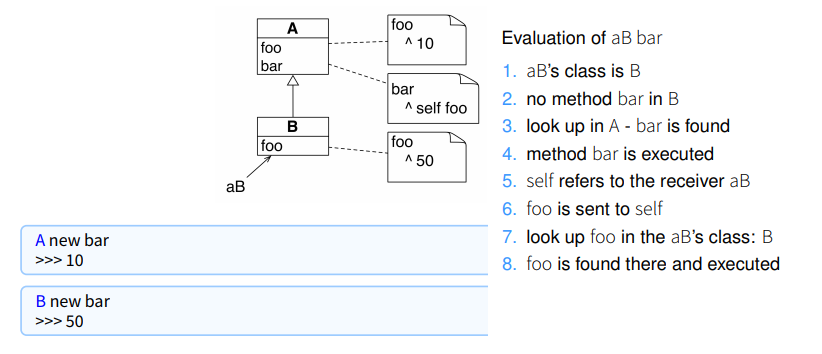
\includegraphics[width=1\textwidth]{topics/bi-wsi-si-09/self.png}
            \caption{Method lookup pro \textbf{self}}
      \end{figure}

      \textbf{super} -- reprezentuje příjemce zprávy (úplně stejně jako \textbf{self}). \textbf{Method-lookup}
      začíná v \textbf{superclass} (hierarchicky nadřazená třída) výrazu, který obsahuje \textbf{super}.

      \begin{figure}[h]
            \centering
            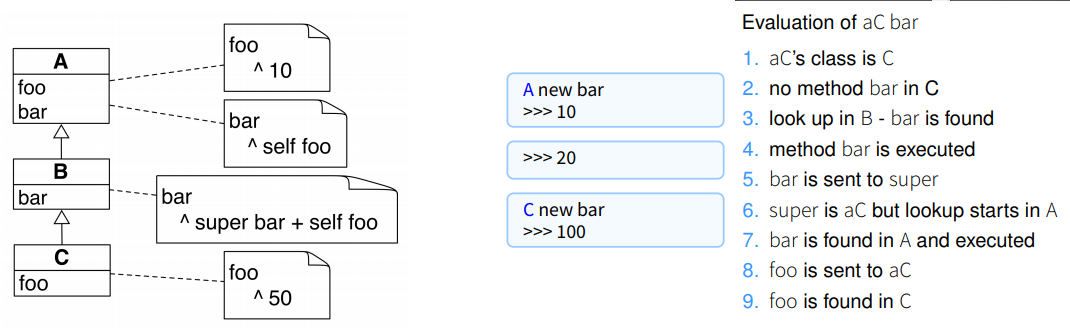
\includegraphics[width=1\textwidth]{topics/bi-wsi-si-09/super.png}
            \caption{Method lookup pro \textbf{super}}
      \end{figure}
      
      \item \textit{Why can we say that sending a message is making a choice?}
      
      Volba prováděné metody odpovídající zasílané zprávě je závislá na příjemci (konkrétní instanci třídy).
      S každým zasláním zprávy tedy \textit{vybíráme} metodu podle aktuálního příjemce.
      To odpovídá \textit{if, then, else} rozhodování, jehož větve se ale vytváří až za běhu programu.

      \item \textit{How 'not' is implemented? What the implementation illustrates?}
      
      \textbf{Boolean} je implementován jako abstraktní třída. Od \textbf{Boolean} dědí třídy \textbf{True}
      a \textbf{False}. Tyto třídy implementují metody \textbf{not}, která pouze vrací instanci toho opačného booleanu.
      Třídy \textbf{True} a \textbf{False} mají singleton instance \textbf{true} a \textbf{false}.

      \begin{figure}[h]
            \centering
            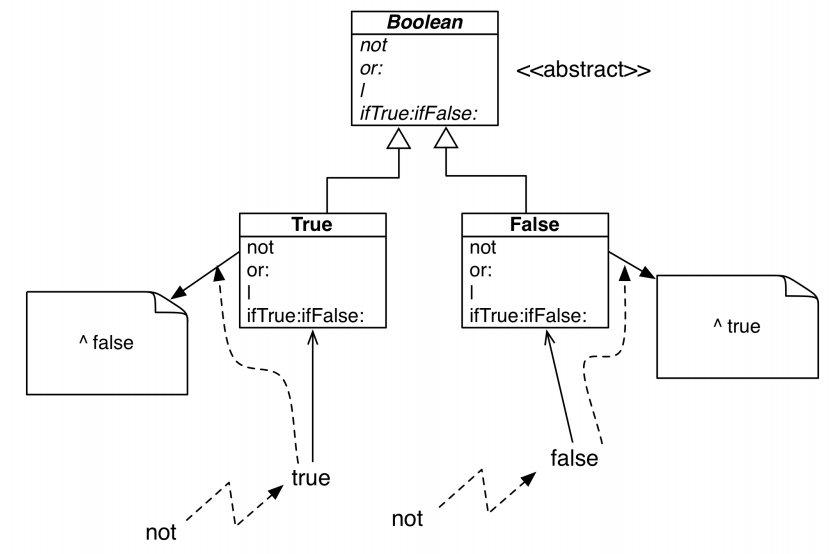
\includegraphics[width=1\textwidth]{topics/bi-wsi-si-09/not.png}
            \caption{Implementace \textbf{not}}
      \end{figure}

      \item \textit{Why is testing important?}
      
      \begin{itemize}
            \item Specifikace očekávaného chování a výsledků (v jistém smyslu slouží i jako dokumentace).
            \item Nalezení problémů a porozumění kódu.
            \item Zvýšení důvěry v kód.
            \item Odhalení bugů, které se projeví změnou jené části kódu.
            \item Izolování problému.
            \item \textit{Další nápady na tuto velice obecnou otázku viz BI-SI1, BI-SI2.}
      \end{itemize}

      Testy by měly:

      \begin{itemize}
            \item ověřit mezní hodnoty,
            \item ověřit komplexní scénáře,
            \item mít dobré pokrytí,
            \item ověřit abstrakci problémů,
            \item být nezávislé.
      \end{itemize}

      \item \textit{Object initialization practices}
      
      \textbf{Provider responsibility} -- je povinností každé třídy aby poskytovala \textit{well-formed} instance,
      tedy takové instance, které nevyžadují žádné další zasílání zpráv pro svoji inicializaci.
      K tomu je důležitá \textbf{automatická inicializace} instančních proměnných a vnitřního stavu obecně,
      například pomocí poskytntí výchozích (\textit{default}) hodnot.

      \textbf{Lazy initialization} -- pozdržení inicializace hodnoty do doby, kdy je hodnotu poprvé potřeba použít.
      Vhodné použít v případě, že nejsou instanční proměnné používané 
      pořád a zabírají spoustu místa nebo závisejí na jiných komponentách.

      \textbf{Zakázání výchozího konstruktoru} -- pokud k vytvoření třídy vždy potřeba nějaký parametr,
      je třeba zabránit vytvoření instance pomocí výchozího konstruktoru, například pomocí vyhození výjimky
      ve vlastní implementaci výchozího konstruktoru.

      \item \textit{Why self-sends are plans for reuse?}
      
      Používání odkazování na příjemce pomocí \textbf{self} v metodách zachovává informaci o třídě instance
      příjemce. To vede k většímu znovupoužití kódu (měníme pouze malé metody v podtřídách a hlavní metoda
      nadtřídy může zůstat jednoduchá).

      \begin{minted}[breaklines]{smalltalk}
      ClassA>>doStuff
      ^ self getNum

      ClassA>>getNum
      ^ 10

      ClassB>>getNum
      ^ 20

      ClassB new doStuff.   " >>>> 20 "
      \end{minted}

\end{itemize}


\end{document}
